\documentclass[a4paper]{article}
\usepackage{array}  
\usepackage[table]{xcolor}% http://ctan.org/pkg/xcolor
\usepackage{geometry}
\geometry{margin=1.25in}
\usepackage{hhline}
\usepackage{environ}
\usepackage{graphicx}
 %\geometry{
 %a4paper,z
 %total={170mm,257mm},
 %left=40mm,
 %right=40mm
 %}
 \newcommand{\colWidth}{141mm}

\begin{document} 
\section*{Demo day: \textit{3} Group \textit{18}}

% ------------GOALS----------

\begin{center}
\begin{tabular}{|p{\colWidth}|}
	\hline
	\cellcolor{blue!25}\large
	\textbf{What were your goals?}
	\\ \hline
	
	\begin{itemize}
		\item Web server 
		\begin{itemize}
			\item Alexa support
			\item Endpoint for unlocking/locking bolt lock
			\item Become an OAuth provider
		\end{itemize}
		\item Android
		\begin{itemize}
			\item UI for unlocking/locking bolt lock
			\item Send request to lock/unlock bolt lock
			\item Use OAuth for authentication
			\item Develop and test a mock-up for a better app UI
		\end{itemize}
		\item Robot
		\begin{itemize}
			\item 3D print light switch grip
			\item Build grip to manipulate bolt lock
			\item Add buttons which allow for manual control of the adapters
		\end{itemize}
	\end{itemize}
	\\ \hline
\end{tabular}
\vskip 5mm

% ------------ORGANISATION----------

\begin{tabular}{|p{\colWidth}|}
	\hline
	\cellcolor{blue!25}\large
	\textbf{Summarise how your group organised the workload to achieve your goals.}
	\\ \hline
	
		We achieved our goals by distributing them across the team in the following manner:
		\begin{itemize}
			\item Web Server:
				\begin{itemize}
					\item Alexa support: Xiaobin, Ben
					\item Endpoint for unlocking/locking bolt lock: Gwion
					\item Become an OAuth provider: Gwion, Ben
				\end{itemize}
			\item Android:
				\begin{itemize}
					\item UI \& server integration for unlocking/locking a bolt lock: thanks to good software architecture, this did not involve making any changes to the app code.
					\item Using OAuth for authentication: Theo
					\item UI mock-up and user testing of this: Ben, Theo
				\end{itemize}
			\item Robot:
			\begin{itemize}
				\item 3D-printing: Luke
				\item Buttons for manual robot control: Spencer
				\item Bolt lock mechanism: Luke
				\item Non-LEGO thermostat design: Han
			\end{itemize}
		\end{itemize}

		As before we are still using GitHub's \textit{Projects} feature to track our progress on the software side, along with communicating on Slack and in our weekly meetings.
		This is the current state of our progress according to the \textit{Projects} tracking feature, in which
		we can easily define \textit{cards} describing tasks to be done, as of 13/3/2019.
		
		\vspace{3mm}
		
		\begin{tabular}{| c || c | c | c |} \hline
			\textbf{Section} & \textbf{Remaining cards} & \textbf{Cards in progress} & \textbf{Finished cards}\\ \hline
			Robot & 1 & 1 & 5 \\
			Web server & 10 & 5 & 11 \\
			Android App & 5 & 1 & 19 \\ \hline
		\end{tabular}

		\vspace{3mm}

		Note that these \textit{cards} do not map directly to our demo goals; for example one of the web server cards is \textit{Create API specification for Smart Home Adapter clients},
		which doesn't lend itself to be targeted for a certain demo as the API specification will need to be changed as we add and modify functionality.
	
  \\
  \hline
\end{tabular}
\vskip 5mm

% ------------ACHIEVEMENTS----------

\begin{tabular}{|p{\colWidth}|}
	\hline
	\cellcolor{blue!25}\large
	\textbf{What were your main achievements?}
	\\ \hline
	\vtop to 95mm{
		Our single biggest achievement for this demo is having OAuth up and running.
		This has been an incredibly large challenge for us, which we initially underestimated as we didn't know we
		needed to be an OAuth \textit{provider} rather than just an OAuth \textit{client}.
		It is largely thanks to the hard work put in by Gwion and Ben over the last couple of weeks that
		we have finally gotten it to work.
		
		\vspace{3mm}
		
		We also managed to finish all the software for interacting with the bolt lock, the UI mock-up along with its user testing, and the buttons for manual control. We are also happy to have managed to conduct a full vulnerability scan of the server.
	}
  \\
  \hline
\end{tabular}
\vskip 5mm

% ------------NOT ACHIEVED----------

\begin{tabular}{|p{\colWidth}|}
	\hline
	\cellcolor{blue!25}\large
	\textbf{What did you not achieve? Briefly explain why.}
	\\ \hline
	\vtop to 95mm{
		We have not managed to reach our "3D printed light switch grip" goal.
		3D printing has once again proven far more time consuming than we expected; we had a
		reasonably good mechanism in place as far back as a week ago, but fine-tuning the
		design is challenging due to the time complexity of iterating designs. In general,
		we were perhaps overtly confident with our new mechanism.
		
		\vspace{3mm}
		
		We have also failed to meet our "bolt lock mechanism" goal. Once again this was due to the
		laborious process of 3D-printing. We have a mechanism printed out that we are confident will work
		-- the fact that the bolt lock does not cause any forces directed back at the robot makes it a lot
		easier than the light switch -- but we did not manage to bring it all together in time.

		\vspace{3mm}

		Finally, we failed to meet our goal of supporting Alexa integration. This was because of how challenging
		it has been to get OAuth up and running, which meant we couldn't test the Alexa skills schema until very,
		very late in the sprint. It is worth saying that we have made really good progress on this and 
		we will have it working very soon, which is quite exciting as it was the feature we thought was most at
		risk of needing to be cut.
		
		\vspace{3mm}
		
		In general, we struggled to meet our goals for this demo despite the group's best efforts.
		Largely this can be attributed to the shorter time allocated to prepare for this demo (2 weeks rather than the 3 weeks we normally have), and the fact that almost all members of the group spent last week working on rather exhausting
		courseworks in Computer Security and Operating Systems.
		
  }
  \\
  \hline
\end{tabular}
\vskip 5mm

% ------------QUANTITIVE----------

\begin{tabular}{|p{\colWidth}|}
	\hline
	\cellcolor{blue!25}\large
	\textbf{Include any quantitative data you have collected (this can be a graph/table with a few words)}
	\\ \hline
	\vtop to 135mm{
		\begin{tabular}{| c || c | c} \hline
			\textbf{Task} & \textbf{Success rate}\\ \hline
			Change thermostat setting & 5/5 \\
			Turn on/off light & 5/5\\
			Rearrange devices & 5/5\\
			Register a new device & 5/5 \\
			Calibrate a new device & 1/5 \\ \hline
		\end{tabular}

		In general the participants struggled to make the connection between the app and the real world. 

		\vspace{3mm}

		Security analysis:
		
		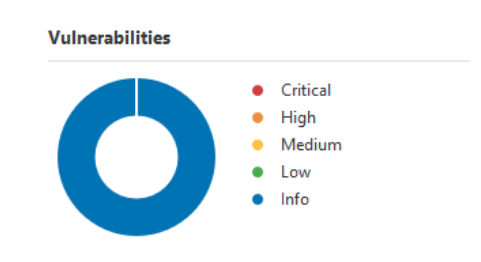
\includegraphics[width=\linewidth]{image.png}
  }
  \\
  \hline
\end{tabular}
\vskip 5mm

% ------------NEXT STEPS----------

\begin{tabular}{|p{\colWidth}|}
	\hline
	\cellcolor{blue!25}\large
	\textbf{Say briefly what changes you will make to your plan for the next demo.}
	\\ \hline
	\vtop to 45mm{
		\begin{itemize}
		\item We may have to cut the \textit{Triggers} feature, to instead allow for more time to polish our existing features (better 3D-printed designs, working PCB, new app design).
	
		\item We will need to spend more time on investigating an alternative solution to the power consumption issue. The ESP8266's do not
		support waking up from deep sleep on packet received, as the deep sleep cuts the WiFi connection.
		This means we cannot make the robot go to deep sleep when not used without manually waking up and
		probing the server every so often, which will lead to high latency.

		\end{itemize}
		
  	}
  \\
  \hline
\end{tabular}

\end{center}
  
\end{document}
